\documentclass[tikz,border=2pt]{standalone}
% Preámbulo común de los diagramas TikZ (misma paleta y letra que las notas)
\usepackage[T1]{fontenc}\usepackage[utf8]{inputenc}
\usepackage{libertinus}\usepackage{libertinust1math}
\usepackage[defaultsans,scale=0.92]{lato}
\usepackage{amsmath,amssymb,bm}
\usepackage{tikz}\usetikzlibrary{calc,positioning,arrows.meta,shapes.geometric,decorations.pathreplacing,decorations.pathmorphing,fit,backgrounds}
\definecolor{snlazul}{HTML}{1E5AA8}\definecolor{snlnoche}{HTML}{14213D}\definecolor{snlvioleta}{HTML}{6C4AB6}
\definecolor{snlcoral}{HTML}{D1495B}\definecolor{snlambar}{HTML}{E09F3E}\definecolor{snlverde}{HTML}{2A9D8F}
\definecolor{snlteal}{HTML}{0F7173}\definecolor{snlgris}{HTML}{5C677D}\definecolor{snlfondo}{HTML}{F4F6FA}
\tikzset{>={Stealth[length=2.2mm]},
  bloque/.style={draw=#1,fill=#1!8,thick,rounded corners=2pt,minimum height=11mm,minimum width=20mm,align=center,font=\small},
  bloque/.default=snlazul,
  suma/.style={draw=snlnoche,thick,circle,inner sep=0pt,minimum size=5mm},
  flecha/.style={->,thick,draw=snlnoche},
  etq/.style={font=\small,text=snlnoche},
  nota/.style={font=\footnotesize\sffamily,text=snlgris,align=center}}

\begin{document}
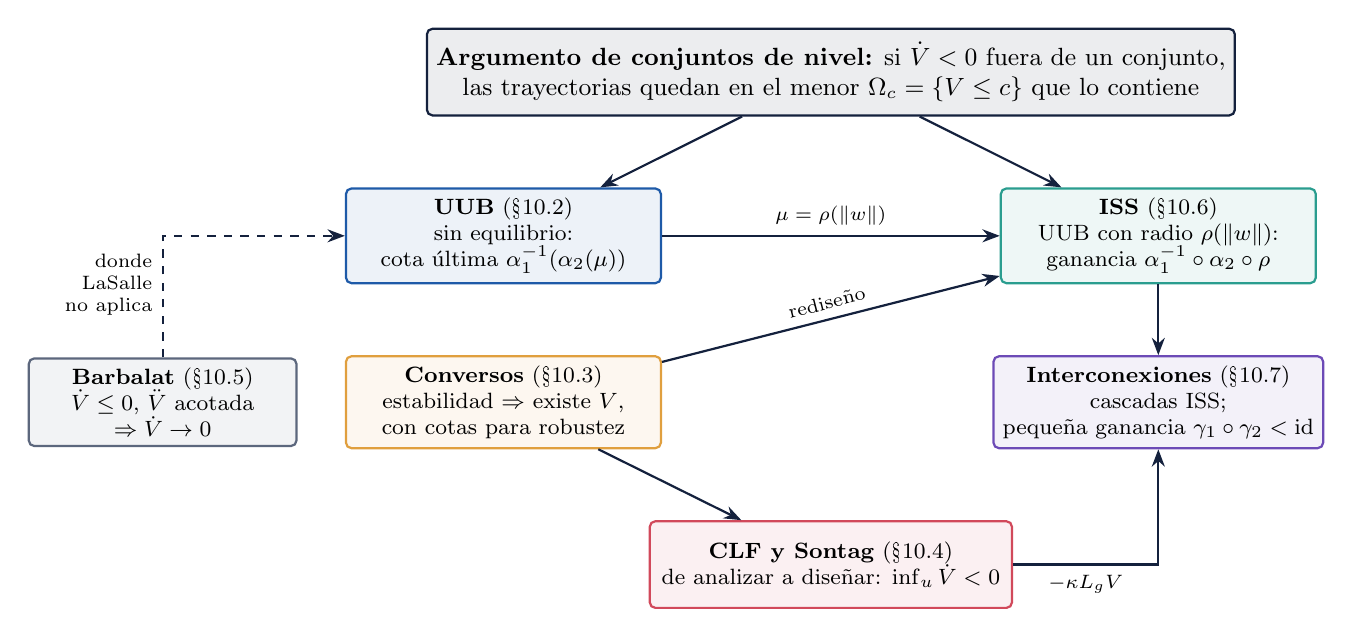
\begin{tikzpicture}[node distance=6mm and 8mm]
 \node[bloque=snlnoche,minimum width=100mm] (arg) {\textbf{Argumento de conjuntos de nivel:} si $\dot V<0$ fuera de un conjunto,\\ las trayectorias quedan en el menor $\Omega_c=\{V\le c\}$ que lo contiene};
 \node[bloque=snlazul,below left=9mm and -30mm of arg,minimum width=40mm,font=\footnotesize] (uub) {\textbf{UUB} (\S10.2)\\ sin equilibrio:\\ cota última $\alpha_1^{-1}(\alpha_2(\mu))$};
 \node[bloque=snlverde,below right=9mm and -30mm of arg,minimum width=40mm,font=\footnotesize] (iss) {\textbf{ISS} (\S10.6)\\ UUB con radio $\rho(\|w\|)$:\\ ganancia $\alpha_1^{-1}\circ\alpha_2\circ\rho$};
 \node[bloque=snlvioleta,below=9mm of iss,minimum width=40mm,font=\footnotesize] (int) {\textbf{Interconexiones} (\S10.7)\\ cascadas ISS;\\ pequeña ganancia $\gamma_1\circ\gamma_2<\mathrm{id}$};
 \node[bloque=snlambar,below=9mm of uub,minimum width=40mm,font=\footnotesize] (conv) {\textbf{Conversos} (\S10.3)\\ estabilidad $\Rightarrow$ existe $V$,\\ con cotas para robustez};
 \node[bloque=snlcoral,below=9mm of $(conv.south)!0.5!(int.south)$,minimum width=46mm,font=\footnotesize] (clf) {\textbf{CLF y Sontag} (\S10.4)\\ de analizar a diseñar: $\inf_u\dot V<0$};
 \node[bloque=snlgris,left=6mm of conv,minimum width=34mm,font=\footnotesize] (bar) {\textbf{Barbalat} (\S10.5)\\ $\dot V\le0$, $\ddot V$ acotada\\ $\Rightarrow\dot V\to0$};
 \draw[flecha] (arg) -- (uub); \draw[flecha] (arg) -- (iss); \draw[flecha] (iss) -- (int);
 \draw[flecha] (uub) -- node[above,font=\scriptsize]{$\mu=\rho(\|w\|)$} (iss);
 \draw[flecha] (conv) -- (clf); \draw[flecha] (conv) -- node[above,font=\scriptsize,sloped]{rediseño} (iss);
 \draw[flecha] (clf) -| node[pos=0.25,below,font=\scriptsize]{$-\kappa L_gV$} (int);
 \draw[flecha,dashed] (bar) |- node[pos=0.3,left,font=\scriptsize,align=right]{donde\\LaSalle\\no aplica} (uub.west);
\end{tikzpicture}
\end{document}
